\documentclass[a4paper, 11pt]{article}
% Include document style
% Packages
\usepackage{lmodern}
\usepackage{amsmath, amssymb}
\usepackage{graphicx}
\usepackage{xcolor}
\usepackage{hyperref}
\usepackage{geometry}
\usepackage{setspace}
\usepackage{microtype}
\usepackage{csquotes}
\usepackage{booktabs}
\usepackage{longtable}
\usepackage{caption}
\usepackage{listings}
\usepackage{fancyhdr}
\usepackage{titlesec}
\usepackage{tikz}
\usepackage{float}
\usepackage{fontspec}
\usepackage{array}
\usepackage{parskip}
\usepackage{acronym}
\usepackage{../../shared/styles/govuk_colors}

% Page Layout
\geometry{margin=2.5cm}
\setstretch{1.2}

% Hyperref
\hypersetup{
    colorlinks=true,
    linkcolor=link-color,
    filecolor=link-color,
    urlcolor=link-active-color,
    citecolor=link-color,
    pdftitle={Your Title Here},
    pdfauthor={Your Name},
    pdfpagemode=FullScreen,
}


\setmainfont[
    Path=/Users/administrator/Code/latex-documents/shared/styles/fonts/Inter-4.0/,
    Extension=.ttf,
    UprightFont=*-Regular,
    BoldFont=*-Bold,
    ItalicFont=*-Italic,
    BoldItalicFont=*-BoldItalic
]{Inter}

% Listings
\lstset{
    backgroundcolor=\color{listing-background},
    basicstyle=\ttfamily\small,
    breaklines=true,
    frame=single,
    framesep=0.19em,
    rulecolor=\color{listing-rule},
    numbers=left,
    numberstyle=\color{listing-numbers},
    keywordstyle=\color{listing-keyword}\bfseries,
    keywordstyle=[2]\color{listing-keyword-2}\bfseries,
    keywordstyle=[3]\color{listing-keyword-3}\bfseries\itshape,
    identifierstyle=\color{listing-identifier},
    commentstyle=\color{listing-comment},
    stringstyle=\color{listing-string},
}

% Captions
\captionsetup{
    font={stretch=1.2},
    textfont={color=secondary-text-color},
    labelfont=bf,
    skip=4mm,
    singlelinecheck=false,
    justification=centering
    % justification=raggedright
}

% Custom heading styles
\titleformat{\section}
{\normalfont\Large\bfseries\color{brand-color}} % Format for \section
{\thesection}{1em}{}

\titleformat{\subsection}
{\normalfont\large\bfseries\color{brand-color}} % Format for \subsection
{\thesubsection}{1em}{}

\titleformat{\subsubsection}
{\normalfont\normalsize\bfseries\color{brand-color}} % Format for \subsubsection
{\thesubsubsection}{1em}{}

% Optional: Custom spacing for sections
\titlespacing*{\section}
{0pt}{2ex plus 1ex minus .2ex}{1ex plus .2ex}

\titlespacing*{\subsection}
{0pt}{1.5ex plus 1ex minus .2ex}{1ex plus .2ex}

\titlespacing*{\subsubsection}
{0pt}{1ex plus 1ex minus .2ex}{1ex plus .2ex}

% Custom header and footer
\pagestyle{fancy}
\fancyhf{}
\fancyhead[L]{\color{brand-color} Custom Header Left}
\fancyhead[C]{\color{brand-color} Custom Header Center}
\fancyhead[R]{\color{brand-color} Custom Header Right}

% Set the color of the header line
\renewcommand{\headrule}{{\color{brand-color}\hrule width\headwidth height\headrulewidth \vskip-\headrulewidth}}
\renewcommand{\headrulewidth}{0.8pt}  % Thickness of the header line

% Header
\setlength{\headheight}{13.6pt}
\addtolength{\topmargin}{-1.6pt}

% array
% Centered column
\newcolumntype{M}[1]{>{\centering\arraybackslash}m{#1}}
% Top ragged right aligned column
\newcolumntype{R}[1]{>{\raggedright\arraybackslash}p{#1}}




% Header and Footer
\pagestyle{fancy}
\fancyhf{}
\fancyhead[L]{Data Management Plan}
\fancyhead[R]{\thepage}
\fancyfoot[L]{Carrow Morris-Wiltshire}
\fancyfoot[R]{\today}

% Title
\title{Data Management Plan}
\author{Carrow Morris-Wiltshire}
\date{\today}

\begin{document}

\maketitle

\section{Collected Data}

\subsection{Sources}

The data used in this project will be predominantly from secondary digital data sources accessed via API or as the results from simulation runs of existing agent-based models which will be through manual file transfer. Some secondary data will be manually extracted from websites and from meetings with stakeholders.

\subsection{Specific Sources}

Primary data collection through API requests to centralised internet of things (IoT) data repositories, such as the Urban Observatory. Additional API sources include the Open Geography Portal (Office for National Statistics) and the Nomanatim API (Open Street Map).
Table 1 shows sample IoT pedestrian data from the urban observatory’s database. All of the data from the urban observatory uses the same fields regardless of sensor type.

\begin{table}[ht]
    \centering
    \scriptsize
    \begin{tabular}{p{2cm}p{1cm}p{1.5cm}p{3cm}p{5cm}p{1cm}}
        \toprule
        \textbf{dt}         & \textbf{value} & \textbf{veh\_class} & \textbf{dir}             & \textbf{location}                 & \textbf{category} \\
        \midrule
        2022-08-18 02:45:00 & 4              & person              & southwest\_to\_northwest & NclNorthumberlandStSavilleRowWest & flow              \\
        2022-06-11 20:15:00 & 9              & person              & northwest\_to\_southwest & NclNorthumberlandStSavilleRowWest & flow              \\
        2022-03-02 23:15:00 & 9              & person              & northeast\_to\_southeast & NclNorthumberlandStSavilleRowEast & flow              \\
        \bottomrule
    \end{tabular}
    \caption{Randomly sampled records from the urban observatory database}
    \label{tab:flowdata}
\end{table}

\subsection{Licensing}

\begin{itemize}
    \item Urban Observatory data is available under the \href{https://creativecommons.org/licenses/by/4.0/}{CCA4 license}.
    \item Open Street Map data is available under the \href{https://opendatacommons.org/licenses/odbl/}{ODbL license}.
    \item Open Geography Portal data is available under the \href{https://www.nationalarchives.gov.uk/doc/open-government-licence/version/3/}{OGv3 license}.
\end{itemize}

\section{Created Data}

\subsection{Sources}

Data will be created through transformation of collected data. These transformations will take place within notebooks and scripts. The majority of the transformed data will not be stored but will be fully reproducible through rerunning notebooks and scripts. The scripts will be accessible in a repository on my \href{https://github.com/carrowmw}{GitHub} page.

\subsection{Licensing}

The data created by this project (including any scripts and notebooks) will be available through the \href{https://opensource.org/license/mit}{MIT} license.

\section{Metadata Standards}

\subsection{Description}

Adherence to established metadata standards for geospatial and IoT data to ensure consistency, clarity, and compatibility for data processing and analysis. The Newcastle University Research Data standards will be used and can be found \href{https://www.ncl.ac.uk/library/academics-and-researchers/research/rdm/working/organise/?}{here}. Metadata standards will apply to the codebase, written documentation, and created data. A variety of standards will be used for these different data forms.

\subsection{Codebase}

The NERC guidelines will be applied to the following: data that were analysed; data processing methods; version of programming language used; list of libraries and their versions; scripts used; analysis techniques; additional datasets; methods of interpretation (visualisations); starting conditions (seeds) for any stochastic modelling. A README file in each folder as well as accompanying project data dictionary and metadata documents will be provided.
Additionally, the SOLID principles will be followed for creating modules or libraries of code. These apply to object-oriented designs and help to ensure they are understandable, flexible, and maintainable:

\begin{itemize}
    \item S - Single-responsibility principle
    \item O - Open-closed principle
    \item L - Liskov substitution principle
    \item I - Interface segregation principle
    \item D - Dependency inversion principle
\end{itemize}

All code will be written with the intent of it being published as a python package. Any code that needs sharing will be dockerised for maximum compatibility. The codebase will follow the paradigms of functional modularity, object oriented programming, config-driven development.

\subsection{Written Documentation}

For written documentation a logical file structure will be followed, and files will use this naming convention $YYYYMMDD\_AUTHORSINITIALS\_FILENAME$.

\subsection{Created Data}

Created data will follow various metadata guidelines depending on the context of the data. For streaming data, the Urban Observatories metadata standards will be adopted. These apply to the three areas shown in figure \ref{fig:metadata}. The first is static data which relates to information such as the manufacturer of the IoT sensor, and the owner and licensing of the data. The second area is generated metadata, this relates to information about the data stream such as clear definitions for the different fields and how often the stream is refreshed. The last area is professional judgement, this will result from exploratory analysis and modelling, to find the limits of the data’s suitability and utility for a range of tasks.

\begin{figure}[ht]
    \centering
    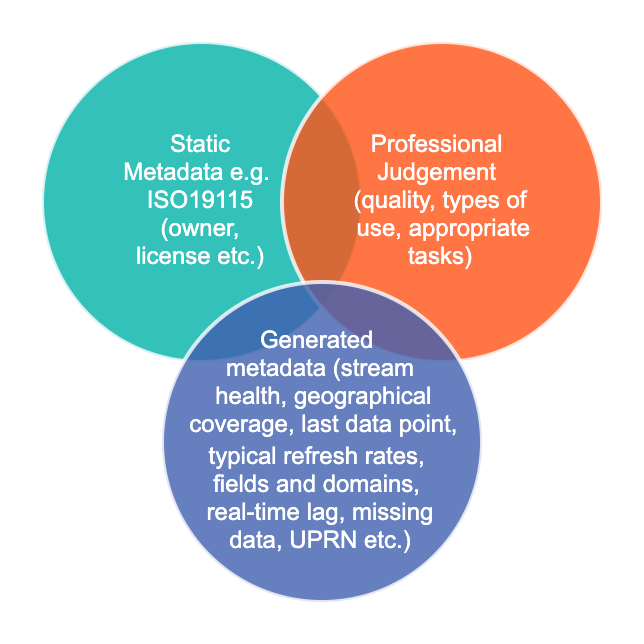
\includegraphics[scale=0.4]{figures/metadata.png}
    \caption{Urban observatory metadata engine for (near) real-time / streaming data}
    \label{fig:metadata}
\end{figure}

\section{Data Structure and Storage}

\subsection{Structure}

Data structure applied to the codebase and created data. The codebase will be structured following style guides of the relevant programming language. For example, PEP 8 and PEP 257 will be followed when using Python. Created data will be stored in the most suitable format for the AI and machine learning algorithms that are used. This will mostly depend on the language and machine learning framework used, for example if models are developed in PyTorch then it makes sense to store data in NumPy arrays or JSON.

\subsection{Storage}

Data storage will utilise secure, scalable cloud storage solutions for data preservation, with appropriate backup and recovery systems. This will involve using Microsoft OneDrive for storing written documents and temporary small datasets, Git will be used for version control of the codebase, which will be periodically pushed to GitHub. Google Cloud Platform will be utilised for storage of large-scale streaming data and model outputs. Cloud service companies offer multiple redundancy so there is no need for further back-up. My personal computer will automatically perform a daily sync with iCloud to ensure that any temporary local files are recoverable.

\section{Data Sharing}

This project is committed to open data principles. This includes publishing in open-access journals where possible, making data free and open for use, and using open-source data ensure that proprietary licenses are not passed down in the process of data transformation. The FAIR principles, guidelines for good data management and stewardship, will be adhered to:

\begin{itemize}
    \item Findable: Data should be easy to find for both humans and computers. Following the metadata guidelines in section 4 will ensure that data is findable.
    \item Accessible: Once found, data must be accessible. Using open-access platforms like GitHub discussed in section 5 ensures data is accessible.
    \item Interoperable: Data should be compatible with other datasets, tools, and workflows for analysis, storage, and processing. Following established frameworks like PyTorch for machine learning ensures that data outputs are interoperable.
    \item Reusable: Data should be well-described and richly documented to enable reuse and replication. Using design and style guides such as SOLID and PEP ensures that data is easily to interpret and manipulate for other users.
\end{itemize}

All significant work will be stored on GitHub and be made publicly available through my \href{https://carrow.me.uk/}{website}.

\section{Data Preservation}

Long-term preservation plans will include clear guidelines on data retention periods and archival methods. Long-term storage will utilise cloud-based platforms (e.g., Google Cloud Platform) to ensure data safety and accessibility over time. Data on GitHub will be held for a period of 10 years post-project completion, with active maintenance for at least the first year. All data will be stored in accessible, non-proprietary formats (e.g., JSON) to facilitate long-term usability.

\section{Ethical Considerations}

All geospatial and IoT data used in the project will comply with data protection laws, such as GDPR. Personal identifiers will be removed or anonymised to protect individual privacy. Potential bias in data collection and algorithm development will be considered. Efforts will be made to ensure that AI models do not perpetuate or amplify existing societal biases. Ethical considerations are covered in more depth in the responsible research and innovation plan.

\section{Responsibility}

\subsection{Management}

Carrow Morris-Wiltshire will be responsible for:
\begin{itemize}
    \item Implementing and updating the DMP.
    \item Data collection, processing, and analysis.
    \item Ensuring data publication and public access at the project end (this includes managing any resource requirements).
\end{itemize}

\subsection{Oversight}

Reviews and audits will be periodically carried out to ensure adherence to the data management plan and compliance with legal and ethical standards. These will occur annually prior to progress review meetings and will involve external review.

\end{document}